%!TEX root = ../Hardtung_PP_WiSe1920.tex

\section{Diagramming Notation}
\label{sec:conventions}

In order to define the concrete requirements of the planned diagramming program, all commonly used diagramming symbols and conventions have to be collected and categorized. After that groundwork a plan can be established on how to implement these findings in a desktop application.

The very fundamentals of Origami diagramming were developed and proposed by Akira Yoshizawa in his book \emph{Atarashi Origami Geijutsu (New Origami Art)}\cite{Yoshizawa} in 1954, which introduced a system of folding notation. Yoshizawas diagramming system is still widely used today and after refining by Samuel Randlett and Robert Harbin most commonly known as the \emph{Yoshizawa–Randlett system}. Despite its high popularity, different nuances and slight changes were made by different origami diagrammers over the years.

To avoid further confusion, especially for beginners, american physicist and origami artist Robert J. Lang compiled notations that were in use by different folders and proposed a standard for all different folding sequences. In order to support his claims, Lang sent \enquote{a questionnaire to 25 diagrammers around the world}\cite{Lang} and tried to coherently argue in favour of, or against the various results. Langs efforts were made under the assumption, that \enquote{[...] unless there is pressing reason otherwise, we should use the standard notation developed by Yoshizawa} \cite{Lang}.

To start off we have to define what exact components a diagram consists of. Most importantly, there always is a visual representation of the paper in the current step. This representation should show all or most creases, flaps, edges and layers to accurately show how the actual paper model would look like (see Section \ref{sec:generalRules} on exceptions).

Secondly, there has to be a description of the actual folding sequence for one step. This description is comprised of a textual explanation and a visual display of the step with the diagramming symbols (Section \ref{sec:notation}). Both the verbal and the visual instructions should be able to stand for themselves, although that might not always be possible for complex steps. More detailed rules and specific terms for the verbal instructions are described in the following Section.

\newpage
\subsection{General Diagramming Rules}
\label{sec:generalRules}

The following rules are general factors to keep in mind when creating origami diagrams. Some aspects here are not necessarily fulfilled by a specific feature within the planned program, but rather depend on the experience of the designer. Though they are still included here as the planned system could offer functions that assist in upholding or at least remind of these rules.

\subsubsection*{Be consistent}
For consistency's sake the artist should stick with one notation within a diagram. One example would be the different ways to symbolize a \gls{mountainFold}. This type of fold results when folding one part of the paper behind the other. After unfolding, the created crease sticks upwards and thus represents a mountain (folding in the other direction results in a \gls{valleyFold}). These mountain folds can either be drawn by a \emph{dash dot} line or by a \emph{dash dot dot} line.

\subsubsection*{Use the right origami grammar}
As earlier established there should be an explanatory text for each folding step. But in order to precisely and clearly describe a fold a consistent grammar has to be used. An important rule is defined by R. Lang: \enquote{origami nouns are not hyphenated, but verbs are} \cite{Lang}. This means that someone \emph{reverse-folds} a flap into the interior but on the other hand flattens out a reverse fold.

Furthermore one should capitalize only those origami moves that \enquote{[...] incorporate names, such as Elias-stretch (verb) or Elias stretch (noun) [...]} \cite{Lang}. The common origami bases like the Bird Base, Waterbomb Base or others are to be capitalized entirely.

\subsubsection*{Distort the model to show all the layers}
Slightly distorting the model to show otherwise hidden layers might be one of the most important general rules, as this one aspect hugely increases the readability and clarity of a diagram. Offering as many reference points as possible makes following a diagram easier and reduces confusion.

\subsubsection*{Creases should not contact the edges}
Already existing creases from previous steps should be drawn with a thin, continuous line and \textbf{not} contact the edges of the paper (see Figure \ref{fig:creasesTouchEdge}). The only exception is when the creases go under a layer of paper. In this case the line that represents the crease does touch the edge of the upper layer. This approach increases the claritiy of a diagram by giving an indication over the order of layers.
\begin{figure*}[htbp]
    \centering
    \begin{subfigure}{0.3\textwidth}
        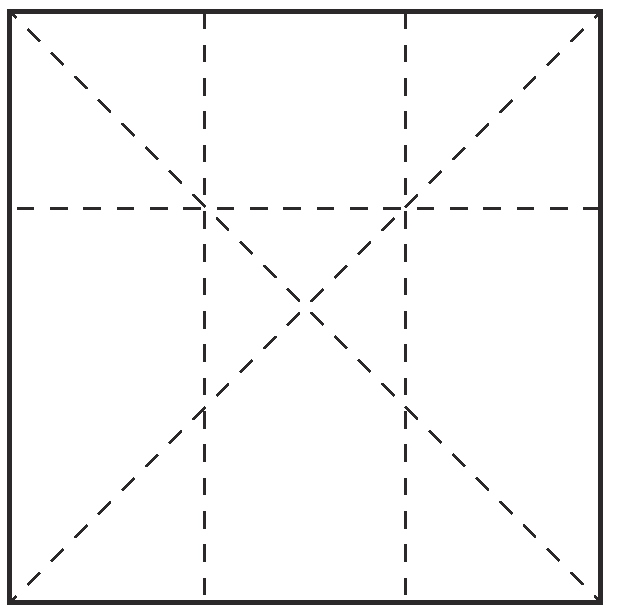
\includegraphics[width=\textwidth]{CreasesTouchEdge1}
        \caption{Folds made}
        \label{fig:creasesTouchEdge1}
    \end{subfigure}
    \begin{subfigure}{0.3\textwidth}
        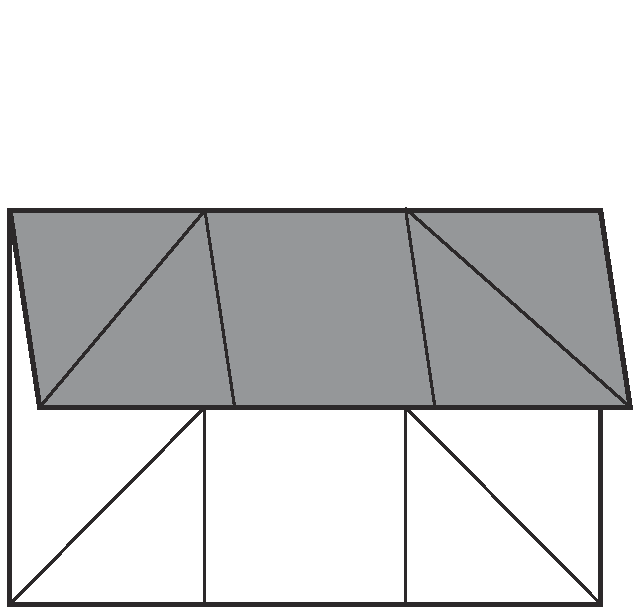
\includegraphics[width=\textwidth]{CreasesTouchEdge2}
        \caption{Wrong way}
        \label{fig:creasesTouchEdge2}
    \end{subfigure}
    \begin{subfigure}{0.3\textwidth}
        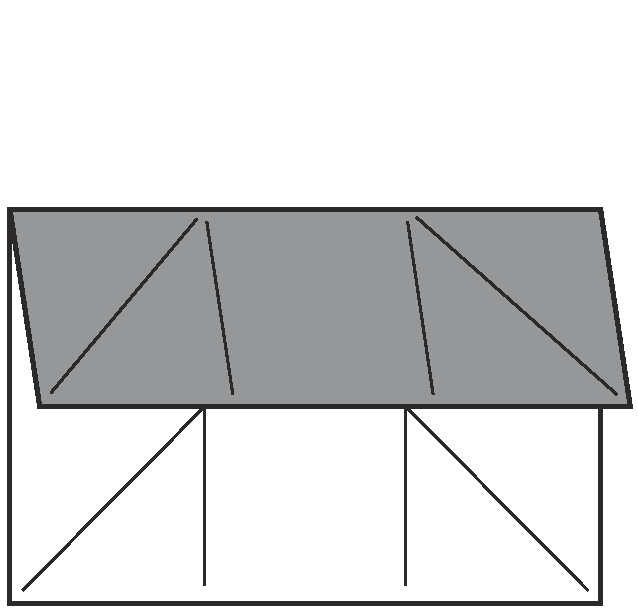
\includegraphics[width=\textwidth]{CreasesTouchEdge3}
        \caption{Correct way}
        \label{fig:creasesTouchEdge3}
    \end{subfigure}
    \caption{How to draw existing creases}\label{fig:creasesTouchEdge}
\end{figure*}

\subsubsection*{Show one white and one colored side of the paper}
When using different colored sides for the paper, the artist can create clearer diagrams. Especially once the instructions get more complex, every additional reference point is helpful.

\subsubsection*{Enlarging the model in a step}
Enlarging the view on a model in a specific step can be accomplished by two methods. The first method mentioned by Lang is marking the area of focus with a circle before enlarging the view. This is especially helpful when focusing on smaller parts during shaping, such as the head. Alternatively the model can simply be enlarged, \enquote{because if you've drawn the diagrams neatly, it is obvious when the drawing has changed scale (and most people won't notice it, anyhow)} \cite{Lang}.

\subsubsection*{Show the result of complex folding steps}
When giving complex folding instructions for a single step (especially when these folds get unfolded in the next step), one should always show the result of said folding sequence. Even though this approach may seem counterproductive as it increases the workload, but once again, the goal is to maximize clarity and remove any ambiguity when creating origami diagrams.

\newpage
\subsection{Diagramming Notation}
\label{sec:notation}

As there are quite a few simple and self-explanatory symbols, there will only be a further explanation if there are any additional rules or things to keep in mind while using them. Furthermore, on occasion Lang gives multiple valid symbols or ways to visualize a certain fold or folding sequence. The goal in these cases should be to give the user a choice on what method to use for a diagram. 

\subsubsection{Folds}
\label{sec:folds}

Starting with the very basics in origami, there has to be a differentiation between the types of folds. Generally, there are 2 different kinds, namely the \gls{valleyFold} and \gls{mountainFold}, which are shown in Figure \ref{fig:valleyFold} and Figure \ref{fig:mountainFold} respectively. Additionally the so called \gls{x-rayLine} is shown in Figure \ref{fig:x-rayLine}. Even though it is not a real fold, it was added here to show the three different forms a line can be drawn in origami diagrams. In order to indicate what kind of fold the X-Ray line is representing, you should extend the line past the paper and use a valley fold or mountain fold line.
\begin{figure*}[htbp]
    \centering
    \begin{subfigure}{0.3\textwidth}
        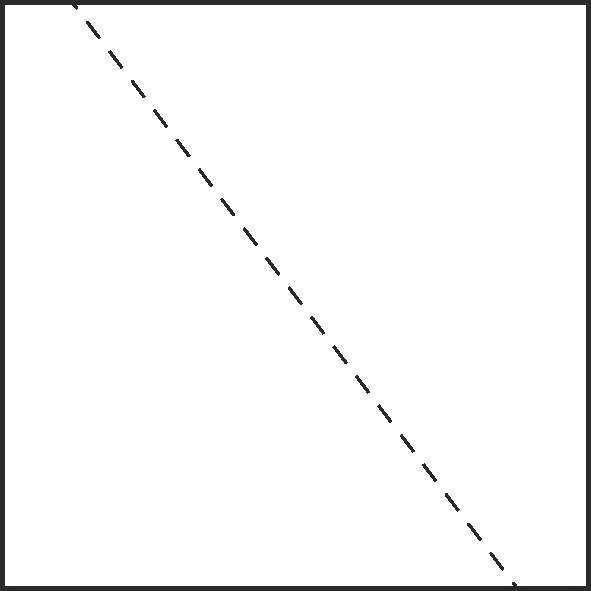
\includegraphics[width=\textwidth]{ValleyFold}
        \caption{Valley Fold}
        \label{fig:valleyFold}
    \end{subfigure}
    \begin{subfigure}{0.3\textwidth}
        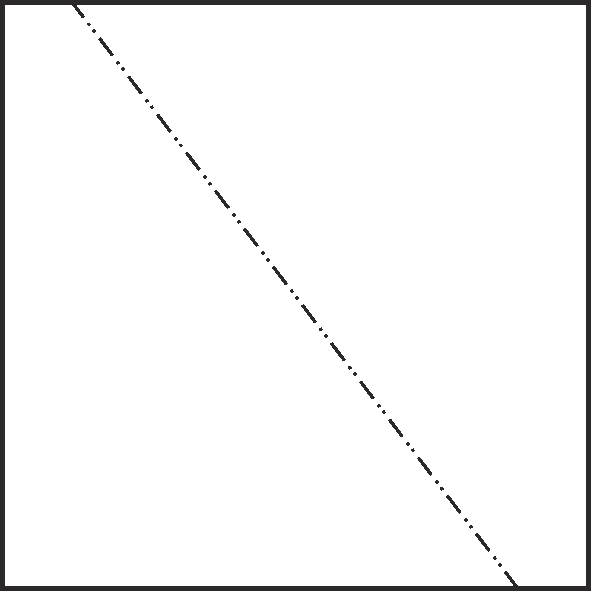
\includegraphics[width=\textwidth]{MountainFold}
        \caption{Mountain Fold}
        \label{fig:mountainFold}
    \end{subfigure}
    \begin{subfigure}{0.3\textwidth}
        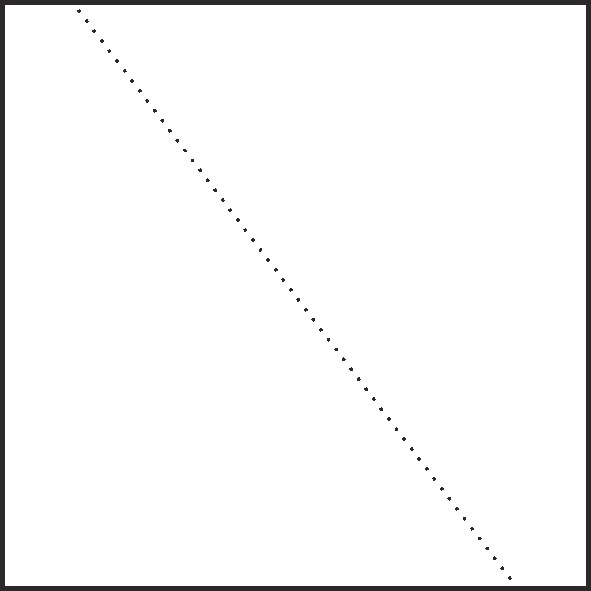
\includegraphics[width=\textwidth]{X-RayLine}
        \caption{X-Ray Line}
        \label{fig:x-rayLine}
    \end{subfigure}
    \caption{Different Lines in Origami Diagramming}\label{fig:origamiLines}
\end{figure*}
\\
Important for the displaying of lines is, that they don't start or end with a gap. This method ensures that there isn't any ambiguity on what reference points are needed for the fold.

\newpage
\subsubsection{Arrows}
\label{sec:arrows}

In order to show the folding steps unambiguously, there have to be arrows that indicate the direction the paper has to be folded. Showing only a valley or mountain fold leaves room for interpretation, which gets eliminated by the addition of these specific arrows. In origami diagramming there are two groups, the \gls{arrowsOfMotion} and \gls{arrowsOfAction}.
While the arrows of motion describe where the paper is folded to, the arrows of action indicate an action perfomed on the paper itself.
\begin{figure*}[htbp]
    \centering
    \begin{subfigure}{0.3\textwidth}
        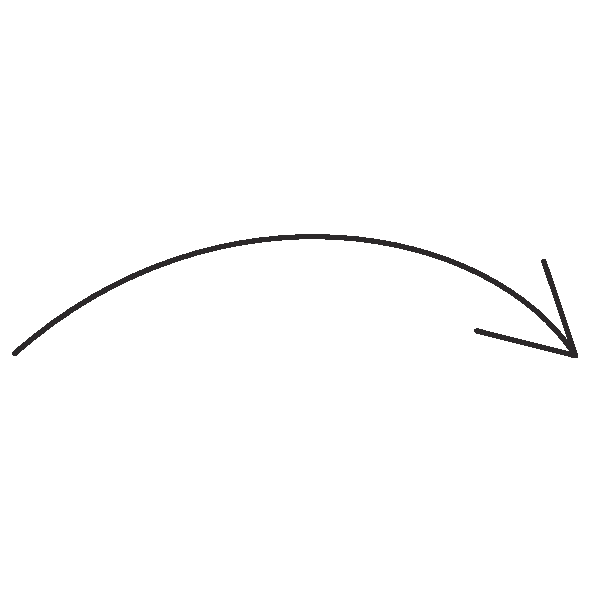
\includegraphics[width=\textwidth]{AoMValleyFold_thick}
        \caption{Valley Fold}
        \label{fig:aomValleyFold}
    \end{subfigure}
    \begin{subfigure}{0.3\textwidth}
        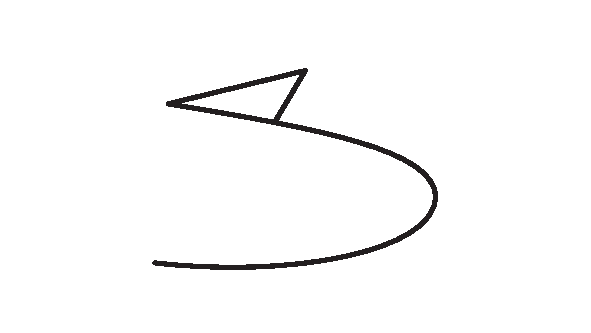
\includegraphics[width=\textwidth]{AoMMountainFold_thick}
        \caption{Mountain Fold}
        \label{fig:aomMountainFold}
    \end{subfigure}
    \begin{subfigure}{0.3\textwidth}
        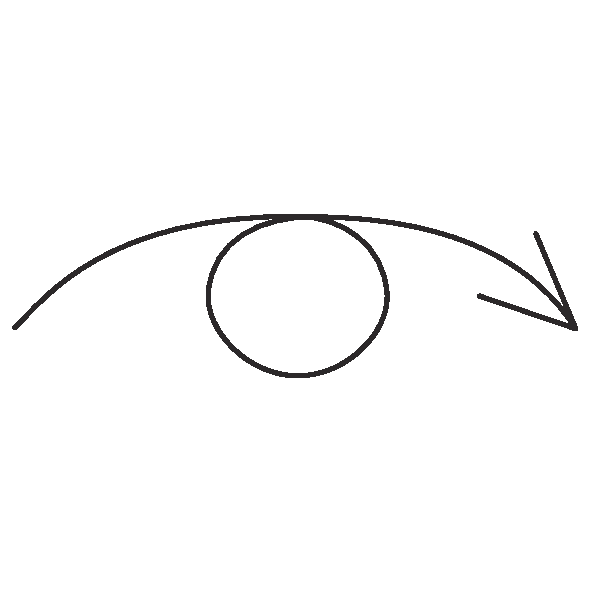
\includegraphics[width=\textwidth]{AoMTurnPaperOver_thick}
        \caption{Turn the paper over}
        \label{fig:aomTurnPaperOver}
    \end{subfigure}
    \caption{Arrows of Motion}
    \label{fig:arrowsOfMotion}
\end{figure*}

\noindent The unfolding arrow can either stand alone and signalize an unfolding action, or be combined with a valley/mountain fold and indicate a folding and unfolding procedure.
\begin{figure*}[htbp]
	\centering
	\begin{subfigure}{0.3\textwidth}
		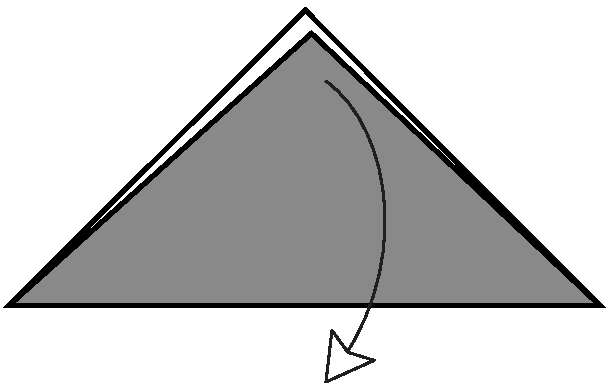
\includegraphics[width=\textwidth]{Unfold}
		\caption{Unfold}
		\label{fig:unfold}
	\end{subfigure}
	\begin{subfigure}{0.25\textwidth}
		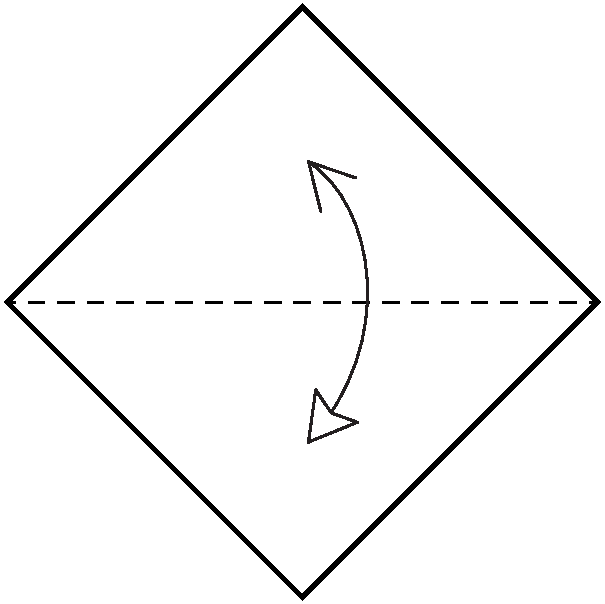
\includegraphics[width=\textwidth]{FoldAndUnfold}
		\caption{Fold and unfold}
		\label{fig:foldAndUnfold}
	\end{subfigure}
	\caption{Unfolding Arrows}
	\label{fig:unfoldingArrows}
\end{figure*}
%
\begin{figure*}[htbp]
    \centering
    \begin{subfigure}{0.3\textwidth}
        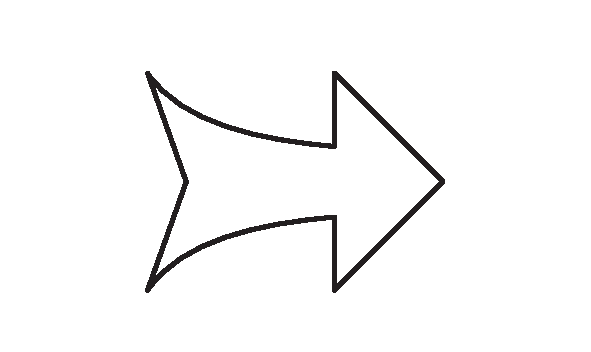
\includegraphics[width=\textwidth]{AoAPushHere_thick}
        \caption{Push here}
        \label{fig:aoaPushHere}
    \end{subfigure}
    \begin{subfigure}{0.3\textwidth}
        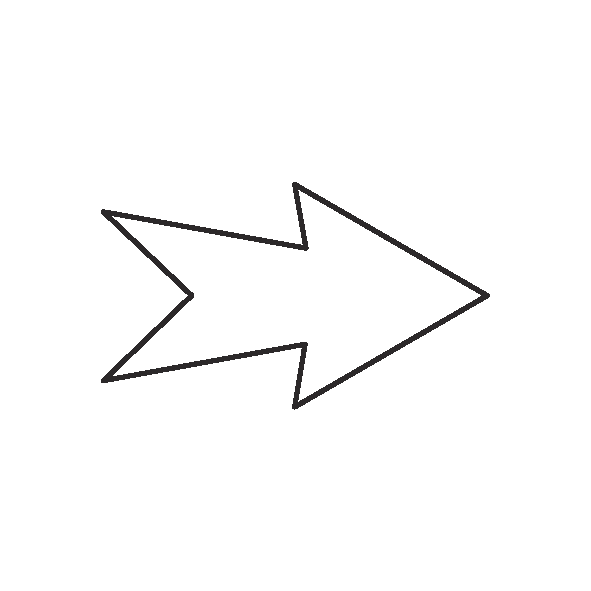
\includegraphics[width=\textwidth]{AoAPullPaperOut_thick}
        \caption{Pull the paper out}
        \label{fig:aoaPullPaperOut}
    \end{subfigure}
    \begin{subfigure}{0.3\textwidth}
        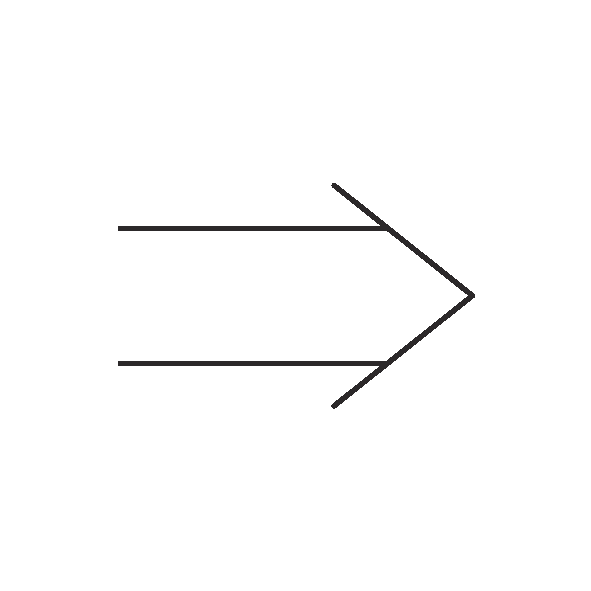
\includegraphics[width=\textwidth]{AoAInflateHere_thick}
        \caption{Inflate here}
        \label{fig:aoaInflateHere}
    \end{subfigure}
    \caption{Arrows of Action}
    \label{fig:arrowsOfAction}
\end{figure*}

\newpage

\subsubsection{Clarifying Diagrams}

\subsubsection*{Leader}
\begin{figure}[htbp]
	\centering
	\def\svgwidth{0.3\textwidth}
	\import{./images/}{Leader.pdf_tex}
	\caption{Use a leader to give additional information if needed}
	\label{fig:leader}
\end{figure}

\subsubsection*{Equal distances}
\begin{figure}[htbp]
	\centering
	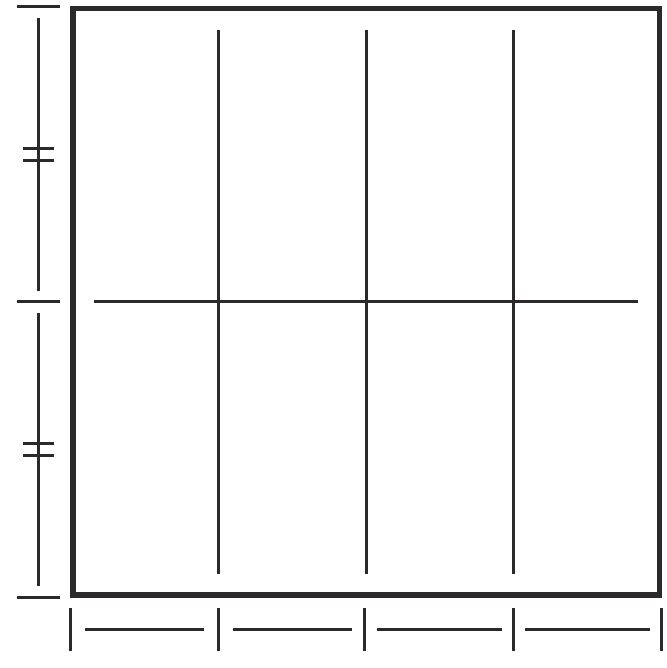
\includegraphics[width=0.3\textwidth]{EqualDistances}
	\caption{Equal Distances}
	\label{fig:equalDistances}
\end{figure}

\subsubsection*{Equal angles}
\begin{figure}[htbp]
	\centering
	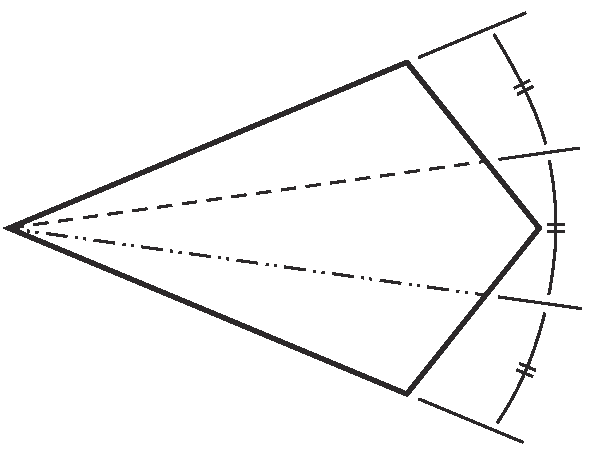
\includegraphics[width=0.3\textwidth]{EqualAngles}
	\caption{Equal Angles}
	\label{fig:equalAngles}
\end{figure}

\subsubsection*{Rotations }
\begin{figure}[htbp]
	\centering
	\def\svgwidth{0.2\textwidth}
	\import{./images/}{Rotation.pdf_tex}
	\caption{Rotation Symbol}
	\label{fig:rotation}
\end{figure}
\noindent The rotation symbol consists of a circle with arrowheads pointing in the rotational direction and a fraction in its center to specify how far to rotate the model.

\subsubsection*{X-Ray View}
\begin{figure*}[htbp]
    \centering
    \begin{subfigure}{0.3\textwidth}
        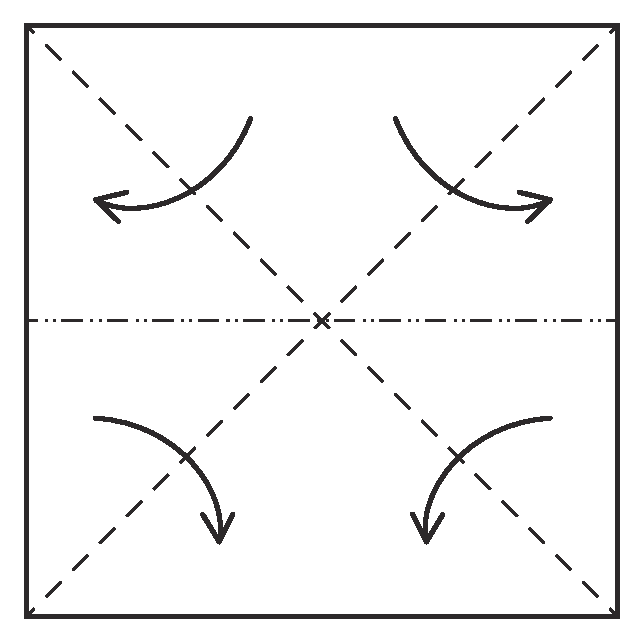
\includegraphics[width=\textwidth]{X-RayViewCP}
        \caption{Folds to be made}
        \label{fig:x-rayViewCP}
    \end{subfigure}
    \begin{subfigure}{0.3\textwidth}
        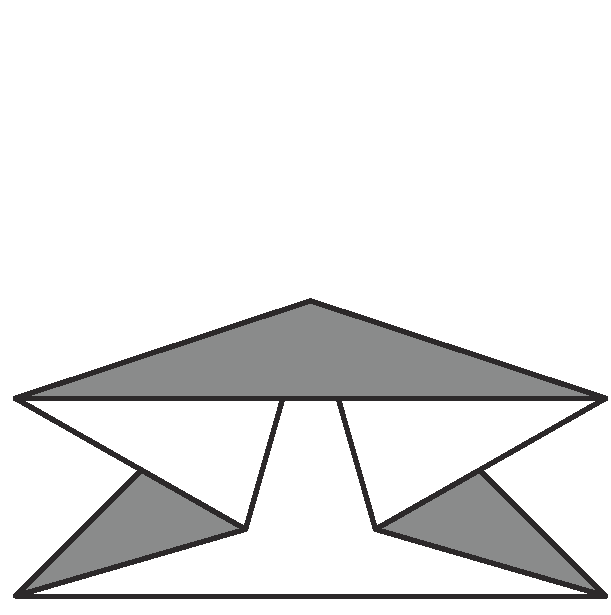
\includegraphics[width=\textwidth]{X-RayViewProcess}
        \caption{Folding Process}
        \label{fig:x-rayViewProcess}
    \end{subfigure}
    \begin{subfigure}{0.5\textwidth}
        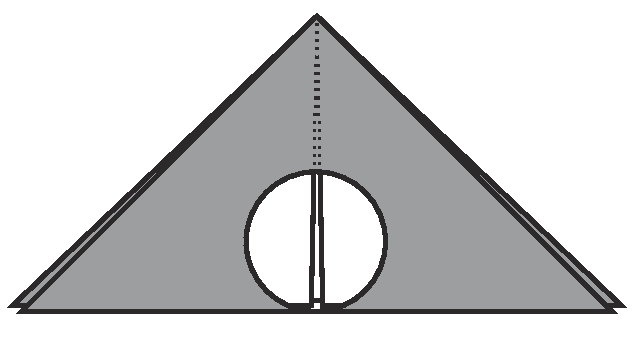
\includegraphics[width=\textwidth]{X-RayView}
        \caption{X-RayView}
        \label{fig:x-rayViewFinal}
    \end{subfigure}
    \caption{X-Ray View}
    \label{fig:x-rayView}
\end{figure*}
\noindent The X-Ray View consists of a circle that removes upper layers of the paper so that hidden layers underneath can be shown.
\newpage
\subsubsection*{Repetitions }

\noindent For complicated repetitions you should show the result of the first fold that is to be repeated.



\begin{figure*}[htbp]
    \centering
    \begin{subfigure}{0.4\textwidth}
        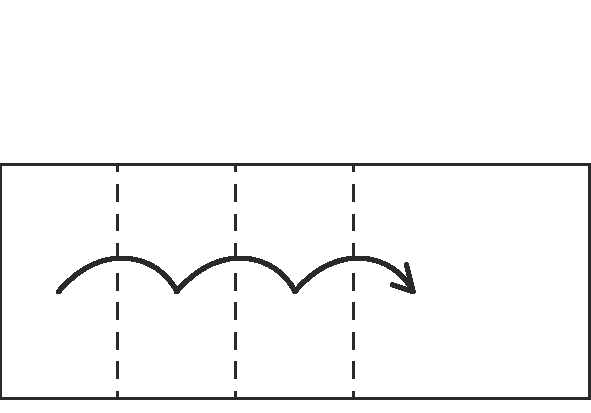
\includegraphics[width=\textwidth]{FoldOverAndOver}
        \caption{Fold Over and Over}
        \label{fig:foldOverAndOver}
    \end{subfigure}
    \begin{subfigure}{0.4\textwidth}
	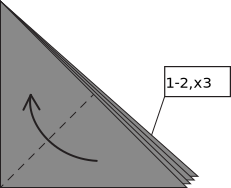
\includegraphics[width=\textwidth]{RepeatBox}
	\caption{Repetition Box}
	\label{fig:repeatBox}
    \end{subfigure}
    \caption{Repetitions}
    \label{fig:holdHerePlusPull}
\end{figure*}

\noindent The repetition box from Figure \ref{fig:repeatBox} shows what exact steps are to be repeated and how many times.

\subsubsection*{Next View Here}
\begin{figure}[htbp]
	\centering
	\def\svgwidth{0.6\textwidth}
	\import{./images/}{NextViewHere.pdf_tex}
	\caption{Next View Here}
	\label{fig:nextViewHere}
\end{figure}

\subsubsection*{Hold Here}
\begin{figure*}[htbp]
    \centering
    \begin{subfigure}{0.3\textwidth}
        \includegraphics[width=\textwidth]{holdHere}
        \caption{Hold Here}
        \label{fig:holdHere}
    \end{subfigure}
    \begin{subfigure}{0.3\textwidth}
        \includegraphics[width=\textwidth]{holdHereAndPull}
        \caption{Hold Here and Pull}
        \label{fig:holdHereAndPull}
    \end{subfigure}
    \caption{Hold Here + Hold Here and Pull Symbols}
    \label{fig:holdHerePlusPull}
\end{figure*}

\newpage
\subsubsection{Folding Procedures}
\subsubsection*{Rabbit Ear}
Lang gives two valid methods to visualize a \gls{rabbitEar}, which is is a folding sequence where you narrow the paper
and create a new flap. This is done by creating three folds at the bisectors of a trigangle. While Figure \ref{fig:rabbitEarA} technically shows the more accurate format (according to the previously defined rules in Section \ref{sec:generalRules}), method B (see Figure \ref{fig:rabbitEarB}) is also desireable, as it shows the overall motion of the paper.
\begin{figure*}[htbp]
    \centering
    \begin{subfigure}{0.27\textwidth}
        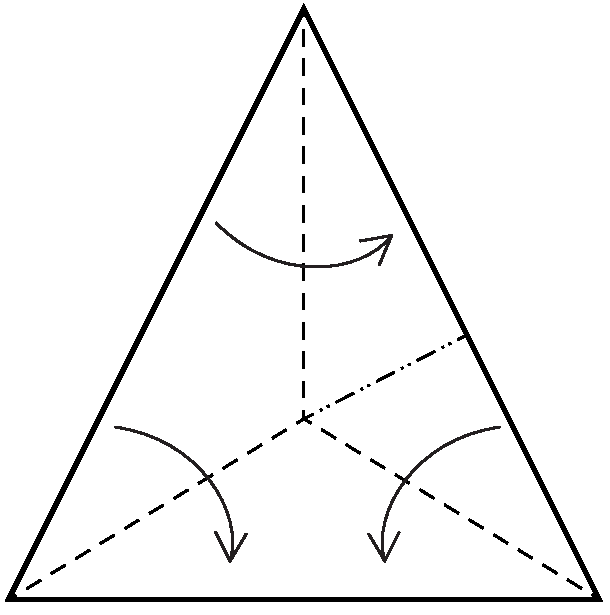
\includegraphics[width=\textwidth]{RabbitEarA}
        \caption{Rabbit Ear A}
        \label{fig:rabbitEarA}
    \end{subfigure}
    \begin{subfigure}{0.35\textwidth}
        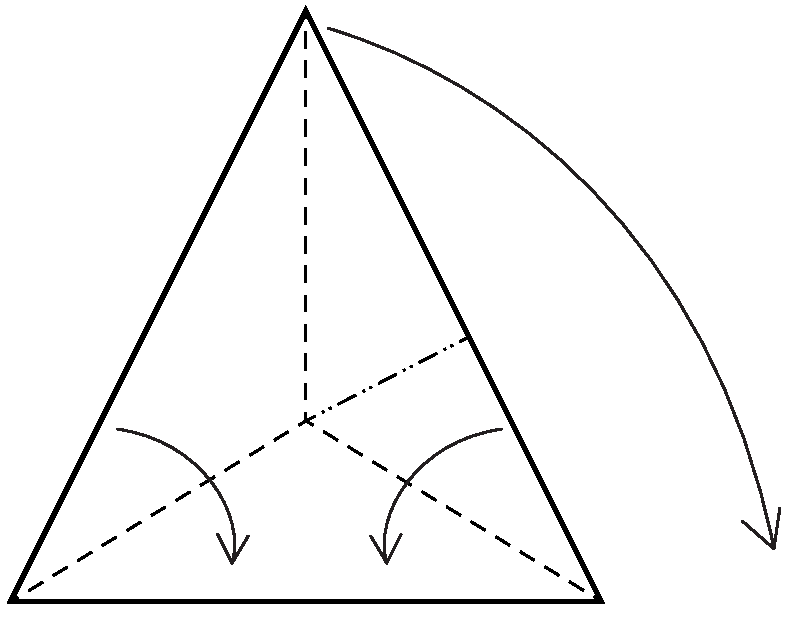
\includegraphics[width=\textwidth]{RabbitEarB}
        \caption{Rabbit Ear B}
        \label{fig:rabbitEarB}
    \end{subfigure}
    \begin{subfigure}{0.33\textwidth}
	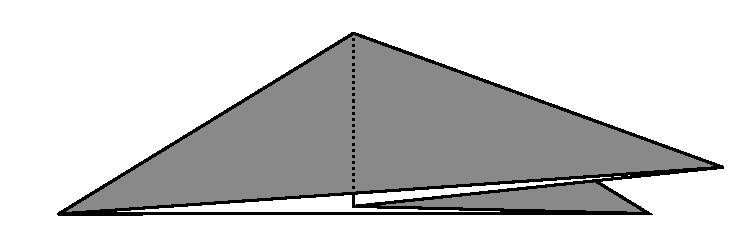
\includegraphics[width=\textwidth]{RabbitEarResult}
	\caption{Rabbit Ear Result}
	\label{fig:rabbitEarResult}
    \end{subfigure}
    \caption{Both methods show a Rabbit Ear Fold}
    \label{fig:rabbitEarMethods}
\end{figure*}

\subsubsection*{Crimping and Pleating}
\begin{figure*}[htbp]
	\centering
	\begin{subfigure}{0.49\textwidth}
		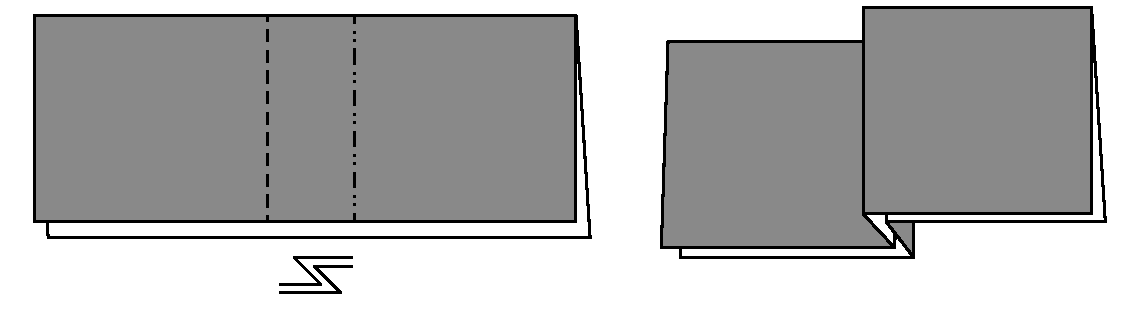
\includegraphics[width=\textwidth]{Crimping}
		\caption{Crimping}
		\label{fig:crimping}
	\end{subfigure}
	\begin{subfigure}{0.49\textwidth}
		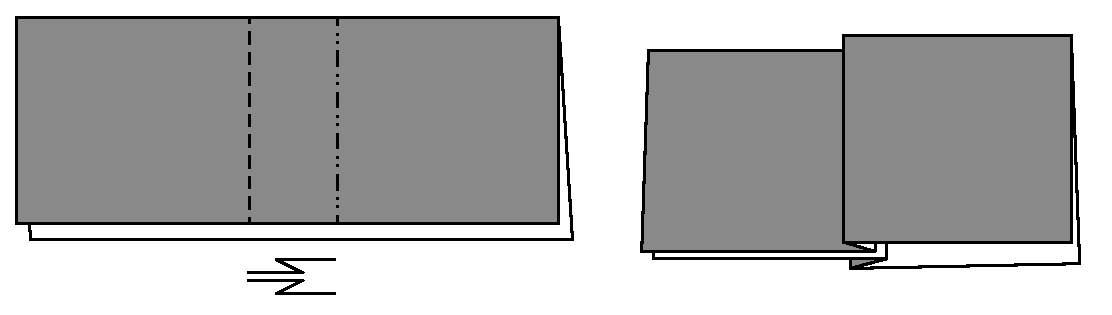
\includegraphics[width=\textwidth]{Pleating}
		\caption{Pleating}
		\label{fig:pleating}
	\end{subfigure}
\end{figure*}

\newpage

\subsubsection*{Reverse Folds}
\begin{figure*}[htbp]
	\centering
	\begin{subfigure}{0.4\textwidth}
		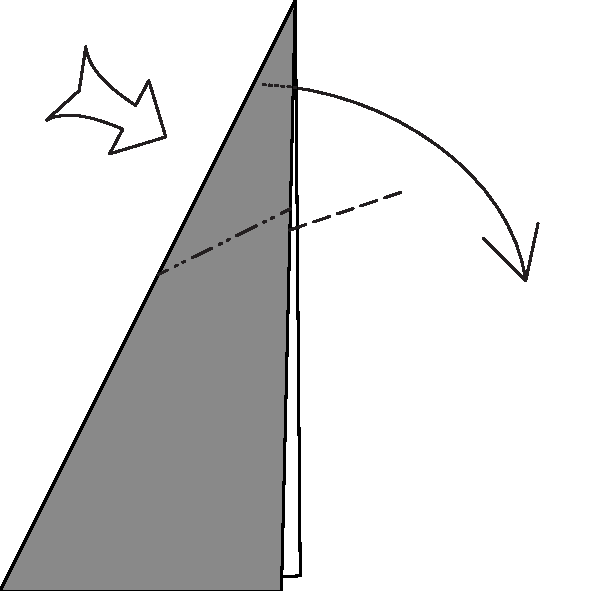
\includegraphics[width=\textwidth]{InsideReverseFold}
		\caption{Notation}
		\label{fig:insideReverseFoldA}
	\end{subfigure}
	\begin{subfigure}{0.4\textwidth}
		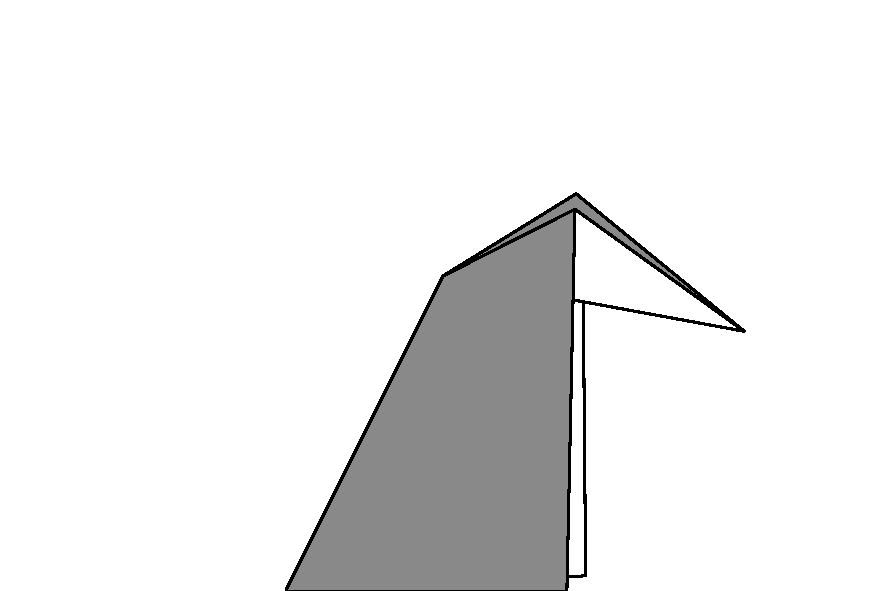
\includegraphics[width=\textwidth]{InsideReverseFoldResult}
		\caption{Result}
		\label{fig:insideReverseFoldResult}
	\end{subfigure}
	\caption{Inside Reverse Fold}
	\label{fig:insideReverseFold}
\end{figure*}
\begin{figure*}[htbp]
	\begin{subfigure}{0.3\textwidth}
		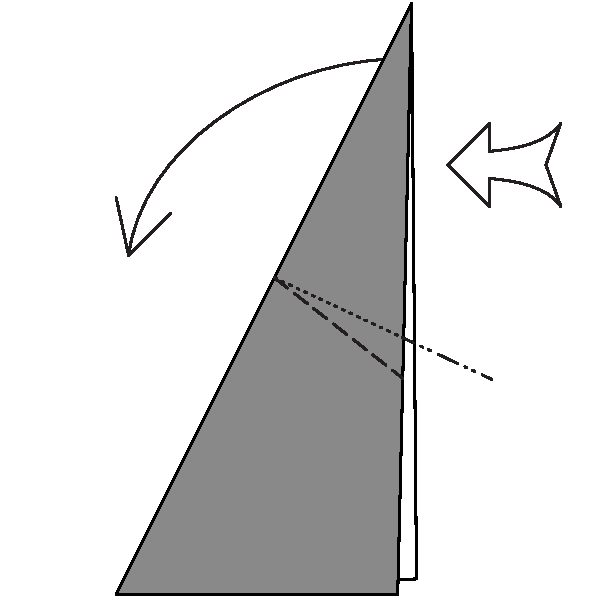
\includegraphics[width=\textwidth]{OutsideReverseFoldA}
		\caption{Notation A}
		\label{fig:outsideReverseFoldA}
	\end{subfigure}
	\begin{subfigure}{0.3\textwidth}
		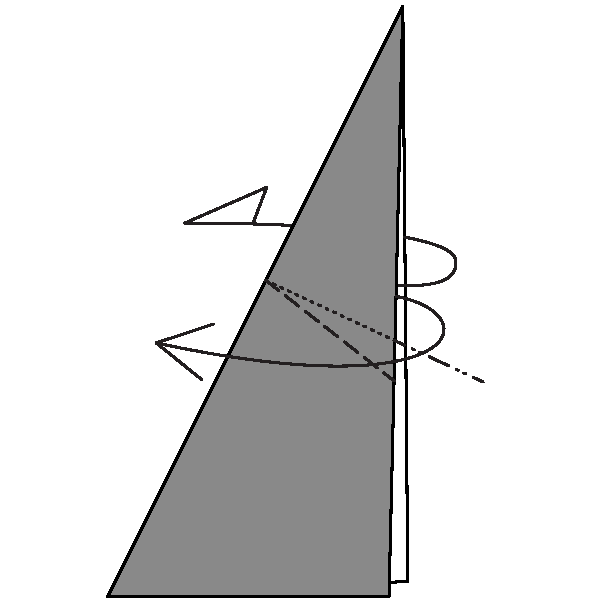
\includegraphics[width=\textwidth]{OutsideReverseFoldB}
		\caption{Notation B}
		\label{fig:outsideReverseFoldB}
	\end{subfigure}
	\begin{subfigure}{0.3\textwidth}
		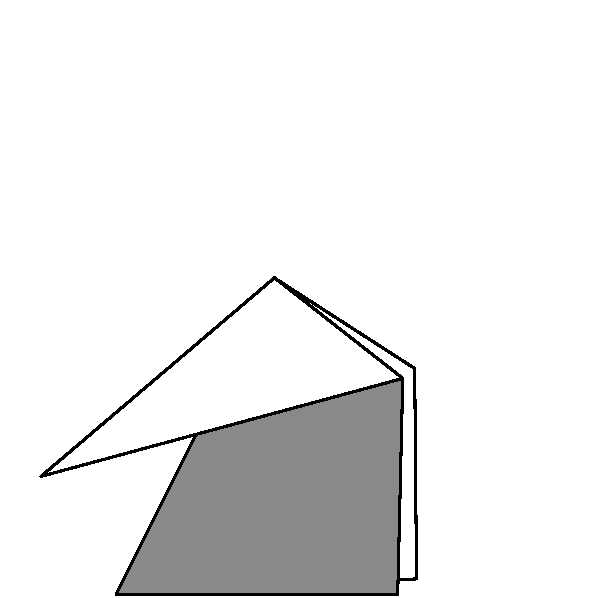
\includegraphics[width=\textwidth]{OutsideReverseFoldResult}
		\caption{Result}
		\label{fig:outsideReverseFoldResult}
	\end{subfigure}
	\caption{Outside Reverse Fold}
	\label{fig:outsideReverseFold}
\end{figure*}
\noindent Although Lang proposes two valid notations for Outside Reverse Folds, for consistency's sake Notation A should be used (see Figure \ref{fig:outsideReverseFoldA}).

\newpage
\subsubsection*{Sinks}
\begin{figure*}[htbp]
	\centering
	\begin{subfigure}{0.7\textwidth}
		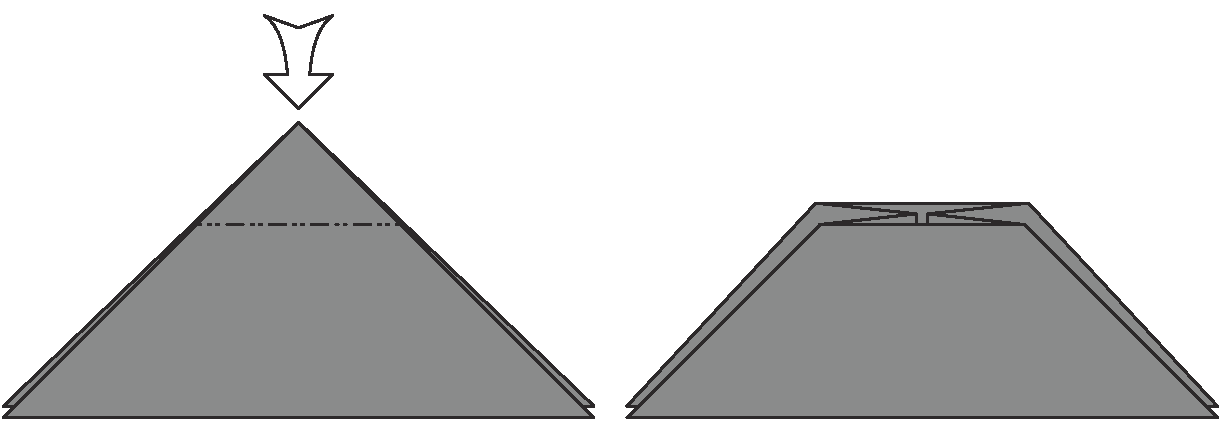
\includegraphics[width=\textwidth]{OpenSink}
		\caption{Open Sink}
		\label{fig:openSink}
	\end{subfigure}
	\begin{subfigure}{0.7\textwidth}
		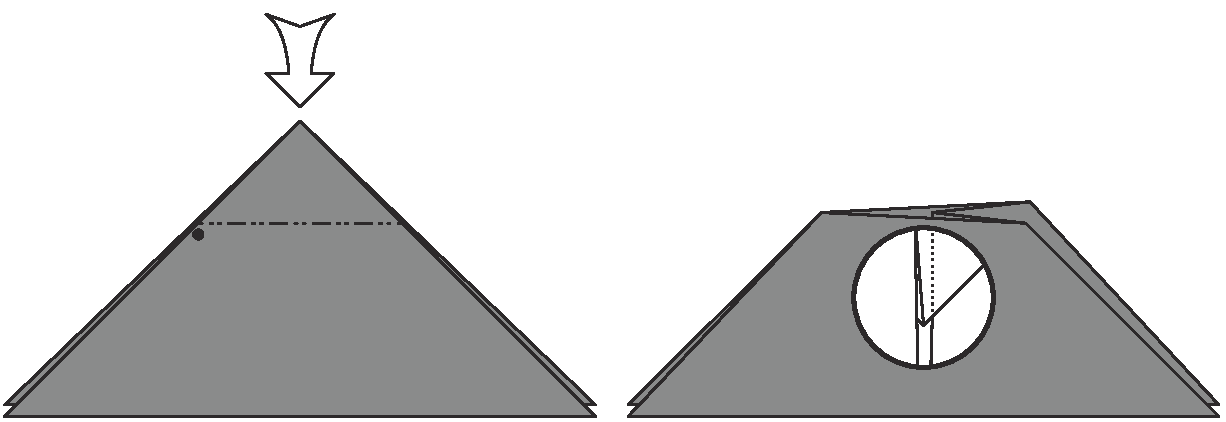
\includegraphics[width=\textwidth]{MixedSink}
		\caption{Mixed Sink}
		\label{fig:mixedSink}
	\end{subfigure}
	\begin{subfigure}{0.7\textwidth}
		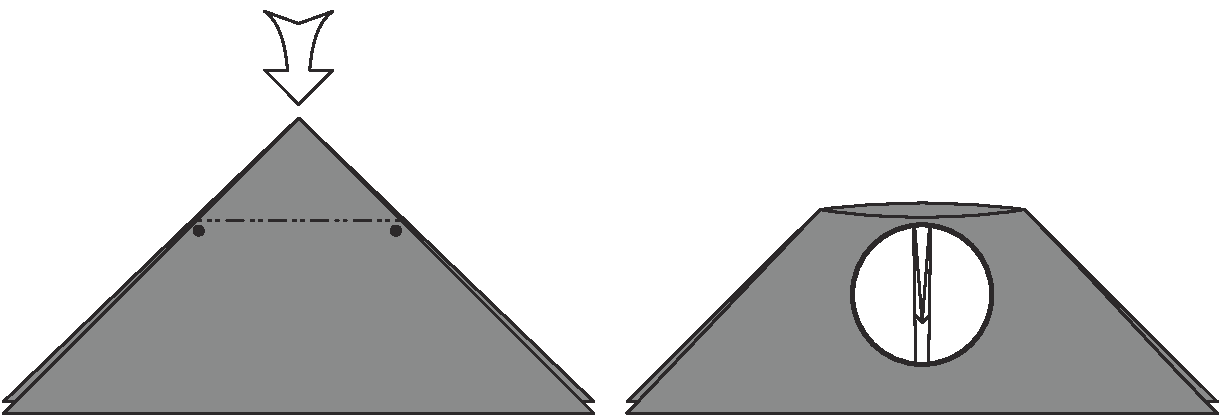
\includegraphics[width=\textwidth]{ClosedSink}
		\caption{Closed Sink}
		\label{fig:closedSink}
	\end{subfigure}
\end{figure*}